\chapter{Implementación Cuántica: Algoritmo QWord2Vec}

En el capítulo anterior se describió en detalle el algoritmo Word2Vec clásico y su variante Skip-gram, que emplea redes neuronales superficiales para aprender representaciones vectoriales de palabras a partir de grandes corpus de texto. En este capítulo se presenta \textit{QWord2Vec}, una adaptación cuántica de dicho modelo propuesta por Ohno \cite{ohno_qword2vec_2025}, cuyo objetivo es explorar si el uso de circuitos cuánticos paramétricos puede ofrecer ventajas en la calidad de las representaciones vectoriales de palabras.

En este capítulo se explorarán la arquitectura del circuito cuántico, la función de coste empleada para su optimización y la estrategia híbrida clásico-cuántica utilizada durante el entrenamiento.

\section{Adaptación del algoritmo al entorno cuántico}

El circuito cuántico de \textit{QWord2Vec} sigue la misma estructura de Word2Vec, compuesta por una parte de \textbf{codificación} y una parte de \textbf{decodificación}. Está formado por puertas de rotación de Pauli (unitarias parametrizadas) y puertas de Pauli-X controladas para introducir entrelazamiento, organizadas en una estructura de capas con profundidad de circuito ajustable. Dado un vector \textit{one-hot} como entrada para una palabra y un vector de salida que representa su contexto \cite{ohno_qword2vec_2025}.

\section{Diseño del Circuito Cuántico Parametrizado}

Como se indicó con anterioridad, la arquitectura de \textit{QWord2Vec} mantiene una estructura análoga a la del algoritmo clásico, dividiéndose en una fase de codificación y otra de decodificación. Esta similitud estructural se ilustra en la Figura \ref{fig:resumen_circuito_qword2vec}.

\begin{figure}[h]
  \centering
  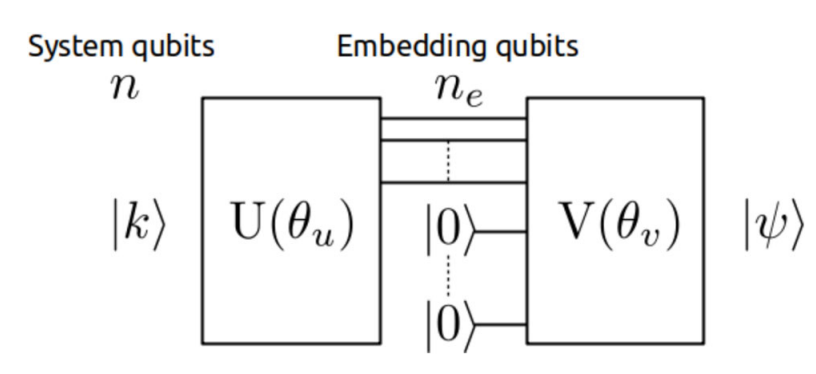
\includegraphics[width=0.9\linewidth]{imagenes/resumenCircuitoQWord2Vec.png}
  \caption{Estructura de QWord2Vec. Fuente: \cite{ohno_qword2vec_2025}.}
  \label{fig:resumen_circuito_qword2vec}
\end{figure}

En la imagen anterior, se aprecia como hay dos matrices parametrizadas, $U(\theta_u)$ y $V(\theta_v)$ junto a una matriz unitaria de entrelazamiento $U(_\text{enta})$. En este sistema, $n$ denota el número total de qubits, mientras que $n_e$ indica el número de qubits destinados específicamente a la representación de los \textit{embeddings}, debiendo cumplirse la restricción $1 \leq n_e \leq n$.

La entrada al circuito viene dada por el estado cuántico $\ket{k}$, el cual representa a una palabra codificada mediante un vector \textit{one-hot}en Word2Vec donde $0 \leq k \leq 2^n - 1$. A partir de este estado inicial, el sistema evoluciona hacia un estado de salida $\ket{\psi}$. Parecido al mapeo directo que realiza Word2Vec, el mapeo que hay entre $\ket{k}$ y $\ket{\psi}$, lo realizan los bloques $U$ y $V$.

Los estados cuánticos de salida resultantes codifican la información correspondiente al contexto de la palabra de entrada, cuya extracción se lleva a cabo realizando mediciones en la base computacional (observable Pauli $Z$).

El modelo $U(\theta_u)$ y $V(\theta_v)$ utilizan las matrices unitarias parametrizadas y las matrices unitarias ($U_\text{enta}$) para proporcionar el entrelazamiento cuántico de la siguiente manera:

\[
  U(\theta) = \prod_{l=1}^{L}
  U_{\text{enta}}\,
  R_Z\!\left(\theta_z^{L-l+1}\right)^{\otimes n}
  R_Y\!\left(\theta_y^{L-l+1}\right)^{\otimes n}
  R_X\!\left(\theta_x^{L-l+1}\right)^{\otimes n}
\]

donde $L$ representa la longitud del circuito cuántico. Por simplicidad, se asumirá que tanto $U(\theta_u)$ como $V(\theta_v)$ poseen la misma profundidad, a menos que se indique explícitamente lo contrario.

Para implementar $U_\text{enta}$, se ha usado puertas controladas Pauli $X$ (CNOT), siguiendo una configuración de circuito por bloques \cite{sim2019expressibility}. Esta disposición favorece notablemente la expresividad del circuito y maximiza su capacidad para generar entrelazamiento. La Figura \ref{fig:qword2vec_circuit} muestra visualmente la estructura del circuito resultante al combinar las rotaciones de Pauli con el bloque de entrelazamiento descrito.

\newpage
\begin{figure}[h]
  \centering
  
\includegraphics[width=1.0\linewidth]{imagenes/qword2vec_circuit.png}
  \caption{Circuito cuántico parametrizado de QWord2Vec con puertas de rotación de Pauli ($R_X$, $R_Y$, $R_Z$) y entrelazamiento con configuración por bloques mediante puertas CNOT.}
  \label{fig:qword2vec_circuit}
\end{figure}

El uso combinado de las tres puertas de rotación ($R_X, R_Y, R_Z$) permite que los estados cuánticos que representan a las distintas palabras alcancen una mayor dispersión en el espacio de Hilbert, superando las limitaciones de representatividad que se obtendrían empleando una sola matriz de rotación, tal y como se observa en la Figura \ref{fig:esferas_bloch_rotaciones_pauli}.

\begin{figure}[h]
  \centering
  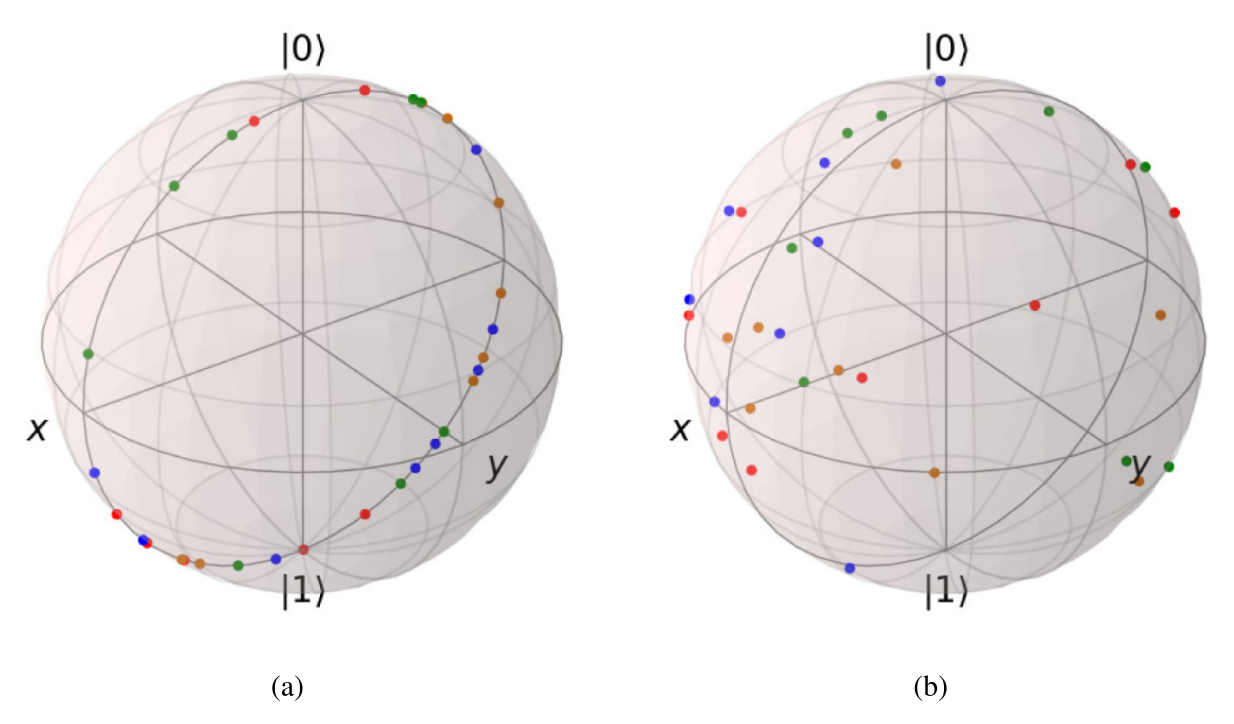
\includegraphics[width=0.9\linewidth]{imagenes/esferaBlochRotacionesPauli.png}
  \caption{Representación de las palabras sobre la esfera de Bloch según las puertas de rotación empleadas en $U(\theta_u)$: (a) usando únicamente $R_Y$, y (b) usando $R_X$, $R_Y$ y $R_Z$ combinadas. Los puntos coloreados corresponden a las palabras y el número total de puntos es 32. El uso de las tres puertas de rotación de Pauli permite una mayor dispersión de las representaciones a lo largo del espacio de Hilbert. Fuente: \cite{ohno_qword2vec_2025}.}
  \label{fig:esferas_bloch_rotaciones_pauli}
\end{figure}

\section{Definición de la función de evaluación y pérdida usadas}

\subsection{Evaluación de los datos de embeddings}

Para evaluar la calidad de los \textit{embeddings} generados por QWord2Vec, se emplea el coeficiente de correlación de Pearson, calculado a partir de las distancias entre los vectores producidos por ambos modelos, Word2Vec y QWord2Vec.

Una vez completado el entrenamiento, se realiza una medición sobre los qubits destinados a los \textit{embeddings}, obteniendo así los vectores clásicos correspondientes a cada palabra. A partir de estos vectores, se construye un \textit{vector distancia}, cuyas componentes son las distancias euclídeas entre los vectores de \textit{embeddings} de todas las palabras del vocabulario. Este proceso se aplica tanto al modelo clásico como al cuántico, tomando el vector distancia de Word2Vec como referencia de comparación (\textit{ground truth}).

El motivo por el que no se utiliza únicamente la entropía cruzada como métrica de evaluación reside en que los circuitos cuánticos con un elevado número de parámetros tienden a reducir su valor. Por ello, se añade el coeficiente de correlación de Pearson sobre los vectores distancia ya que constituye una métrica más adecuada y robusta para valorar la capacidad del modelo. En la siguiente subsección se describe en detalle la función de pérdida empleada durante el entrenamiento del circuito.

\subsection{Función de pérdida}

La función de pérdida usada, además de tener el componente de la pérdida de entropía cruzada, se le añade un término junto al coeficiente de correlación de Pearson. Por lo que la función de pérdida queda de la siguiente manera:

\[
  \text{Loss} := \text{CrossEntropyLoss} - C \cdot \text{CorrelationCoefficient}(\textit{EmbeddingData}, \textit{ReferencesDistances}),
\]

Donde $C > 0$ es un parámetro de balanceo. $\text{CorrelationCoefficient}(\textit{EmbeddingData}, \textit{ReferencesDistances})$ se refiere al coeficiente de correlación entre el vector distancia de los datos de embeddings (\textit{EmbeddingData}) en QWord2Vec el cual se actualiza en cada iteración mientras que \textit{ReferencesDistances}, se refiere al vector de distancias referencias en este caso el obtenido de Word2Vec.




\section{Estrategia de optimización híbrida (Clásica-Cuántica)}

